\documentclass[review]{elsarticle}
\usepackage[utf8]{inputenc}
\usepackage[T1]{fontenc}
\usepackage{amsmath,amssymb}
\usepackage{siunitx}
\usepackage{graphicx}
\usepackage{booktabs}
\usepackage[pdfencoding=auto,psdextra]{hyperref}
\usepackage{lineno}
\graphicspath{{figures/}}
\hypersetup{pageanchor=false}
\AtBeginDocument{\hypersetup{pageanchor=true}}
\sisetup{per-mode=symbol, group-separator={,}}
\linenumbers
\journal{The Journal of the Acoustical Society of America}

\begin{document}
\begin{frontmatter}

\title{What pitch is a growling stomach? A unified multi-mode acoustic model of borborygmi}

\author[msr]{Jonathan Mace\corref{cor1}}
\cortext[cor1]{Corresponding author}
\ead{jonathanmace@microsoft.com}

\author[auckland]{Brian R.\ Mace}
\ead{br.mace@auckland.ac.nz}

\affiliation[msr]{organization={Microsoft Research}, city={Redmond, WA}, country={United States}}
\affiliation[auckland]{organization={Acoustics Research Centre, Department of Mechanical and
    Mechatronics Engineering, University of Auckland}, city={Auckland}, country={New Zealand}}

\begin{abstract}
Borborygmi---the rumbling and gurgling sounds of the gastrointestinal
tract---arise from oscillation of gas pockets entrained in intestinal fluid.
Despite their clinical significance as indicators of gut motility, no
first-principles acoustic model predicts their frequency spectrum from
measurable anatomical parameters.  We present a unified analytical framework
comprising five resonance mechanisms: (i)~free Minnaert bubble oscillation,
(ii)~tissue-constrained bubble resonance incorporating intestinal wall
elasticity, (iii)~Helmholtz resonance through peristaltic constrictions,
(iv)~axial piston modes of cylindrical gas slugs, and (v)~radial breathing
modes of gas columns in elastic tubes.  The constrained bubble model predicts
frequencies of \SIrange{135}{440}{\hertz} for gas pocket volumes of
\SIrange{1}{50}{\milli\litre}, overlapping the clinically observed
\SIrange{200}{550}{\hertz} band for healthy adults without curve-fitting.
A mode-transition map identifies which resonance mechanism dominates in each
region of the volume--geometry parameter space.  The framework provides a
physics-based tool for interpreting auscultatory findings and designing acoustic
monitoring systems for gastrointestinal motility assessment.
\end{abstract}

\begin{keyword}
borborygmi \sep bowel sounds \sep Minnaert resonance \sep bubble acoustics \sep
gastrointestinal acoustics \sep Helmholtz resonator
\end{keyword}

\end{frontmatter}

%% ===================================================================
%% I. INTRODUCTION
%% ===================================================================
\section{Introduction}
\label{sec:introduction}

Few acoustic phenomena are as universally experienced yet as poorly understood
as the sounds of the gastrointestinal tract.  Borborygmi---the medical term
for stomach and intestinal gurgling---have been documented since at least
Cannon's~\cite{Cannon1905} pioneering auscultation studies, and their
clinical significance as indicators of gut motility, obstruction, and
post-operative recovery is well established~\cite{Ching2012, Craine1999,
DalleDonne2024}.  Despite this long history, clinical assessment of bowel
sounds remains largely qualitative: present or absent, normoactive or
hyperactive, high-pitched or low-pitched.

The past two decades have seen growing interest in quantitative bowel sound
analysis.  Craine et~al.~\cite{Craine1999, Craine2002} developed
computerised auscultation systems and reported spectral differences between
normal and obstructed bowel.  Ching and Tan~\cite{Ching2012} performed
spectral analysis using electronic stethoscopes and documented that healthy
bowel sounds occupy a band of approximately \SIrange{200}{550}{\hertz} with
a peak near \SI{340}{\hertz}, while intestinal obstruction shifts the
spectrum in condition-specific ways.  More recently, Nowak
et~al.~\cite{Nowak2021} reviewed automated bowel sound analysis using machine
learning classifiers, and Dalle~Donne et~al.~\cite{DalleDonne2024} surveyed
wearable monitoring systems.  These approaches treat bowel sounds as signals
to be classified, but offer no predictive model explaining \emph{why}
particular frequencies appear.

The physics of bubble acoustics, by contrast, is mature.  The
classical result of Minnaert~\cite{Minnaert1933} for the resonant frequency
of a spherical gas bubble in an incompressible fluid remains the starting
point for underwater and biomedical acoustics alike~\cite{Leighton1994}.
Church~\cite{Church1995} extended the theory to bubbles encapsulated in
elastic shells---primarily for ultrasound contrast agents---and
Hoff~\cite{Hoff2001} provided a comprehensive treatment of coated bubble
dynamics.  Li et~al.~\cite{Li2022} recently derived rigorous Minnaert
corrections for bubbles in soft elastic media, while Ammari
et~al.~\cite{Ammari2018} analysed bubbly media from a mathematical
perspective.  None of these works, however, has been applied to the specific
geometry, material properties, and clinical context of the gastrointestinal
tract.

We bridge this gap.  In this paper we present a unified analytical framework
in which intestinal gas pockets are modelled as acoustically resonant systems,
with five distinct mechanisms producing frequencies that overlap the clinically
observed spectrum.  The model requires no fitted parameters: all inputs are
measurable anatomical and material properties---gas pocket volume, intestinal
wall stiffness, lumen diameter, and constriction geometry---drawn from
published literature or standard anatomical measurements.  The
tissue-constrained bubble mechanism was first analysed in the context of
abdominal resonance by~\cite{Mace2026gaspockets}, whose constrained-bubble
formulation we extend here to the intestinal geometry.  The
tissue-constrained bubble model, which augments the Minnaert formula with
elastic wall stiffness and inertia, captures much of the healthy bowel sound band
of \SIrange{200}{550}{\hertz} for pocket volumes of
\SIrange{1}{50}{\milli\litre}, specifically the \SIrange{200}{440}{\hertz}
sub-band.  Frequencies above \SI{440}{\hertz} likely require sub-millilitre
pockets or Helmholtz contributions.  A mode-transition map reveals which resonance
mechanism dominates in each region of the volume--diameter parameter space,
providing physical insight for interpreting auscultatory findings.

%% ===================================================================
%% II. THEORY
%% ===================================================================
\section{Theory}
\label{sec:theory}

We model a gas pocket of volume $V$ trapped within the fluid-filled lumen of
the intestinal tract.  The pocket is surrounded by incompressible intestinal
fluid of density $\rho_f = \SI{1020}{\kilogram\per\metre\cubed}$ and confined
by an elastic intestinal wall of Young's modulus $E$, Poisson's ratio $\nu$,
thickness $h$, and density $\rho_w$.  Five resonance mechanisms are
considered, each corresponding to a distinct physical geometry and oscillation
pattern.  Table~\ref{tab:params} summarises the canonical parameter values
used throughout.

\begin{table}[t]
\centering
\caption{Canonical parameter values for the borborygmi model.}
\label{tab:params}
\begin{tabular}{llll}
\toprule
Parameter & Symbol & Value & Unit \\
\midrule
Gas adiabatic exponent & $\gamma$ & 1.4 & --- \\
Atmospheric pressure & $P_\mathrm{atm}$ & 101,325 & \si{\pascal} \\
Intra-abdominal pressure & $P_\mathrm{iap}$ & 1,000 & \si{\pascal} \\
Ambient pressure & $P_0$ & 102,325 & \si{\pascal} \\
Intestinal fluid density & $\rho_f$ & 1,020 & \si{\kilogram\per\metre\cubed} \\
Intestinal wall modulus & $E$ & 10 & \si{\kilo\pascal} \\
Wall Poisson's ratio & $\nu$ & 0.45 & --- \\
Wall thickness & $h$ & 3.0 & \si{\milli\metre} \\
Wall density & $\rho_w$ & 1,040 & \si{\kilogram\per\metre\cubed} \\
Lumen diameter & $d$ & 30 & \si{\milli\metre} \\
Gas sound speed & $c_g$ & 343\textsuperscript{a} & \si{\metre\per\second} \\
Neck diameter (Helmholtz) & $d_n$ & 5 & \si{\milli\metre} \\
Neck length (Helmholtz) & $L_n$ & 10 & \si{\milli\metre} \\
Loss tangent & $\eta$ & 0.25 & --- \\
\bottomrule
\end{tabular}
\par\smallskip
\textsuperscript{a}Room-temperature value; air at \SI{37}{\degreeCelsius} gives
$c_g \approx \SI{353}{\metre\per\second}$, a ${\sim}3\%$ difference that
affects only the Helmholtz mode and is smaller than the parametric uncertainty.
\end{table}

\subsection{Free Minnaert bubble}
\label{sec:minnaert}

The classical Minnaert frequency~\cite{Minnaert1933} for radial pulsation of
a spherical gas bubble of radius $R$ in an unbounded incompressible fluid is
\begin{equation}
  f_M = \frac{1}{2\pi R}\sqrt{\frac{3\gamma P_0}{\rho_f}},
  \label{eq:minnaert}
\end{equation}
where $\gamma$ is the polytropic exponent, $P_0$ is the ambient pressure, and
$\rho_f$ is the fluid density.  The equivalent spherical radius is related to
the pocket volume~$V$ by $R = (3V/4\pi)^{1/3}$.  For a
\SI{10}{\milli\litre} pocket ($R = \SI{13.4}{\milli\metre}$) in intestinal
fluid at body temperature, Eq.~\eqref{eq:minnaert} gives
$f_M = \SI{244}{\hertz}$.

The Minnaert frequency provides a useful baseline but neglects the elastic
constraint of the surrounding intestinal wall.  For a bubble suspended in
free fluid this is appropriate; for a gas pocket enclosed within the gut, it
is not.

\subsection{Tissue-constrained bubble}
\label{sec:constrained}

The intestinal wall wrapping the gas pocket contributes both elastic
stiffness and inertia.  Following the approach of Church~\cite{Church1995}
for encapsulated bubbles, we model the wall as a thin elastic shell of
thickness $h$ concentric with the spherical gas pocket.  The restoring force
per unit surface area per unit radial displacement comprises a gas
compressibility term and a wall elasticity term:
\begin{equation}
  k_\mathrm{gas} = \frac{3\gamma P_0}{R}, \qquad
  k_\mathrm{wall} = \frac{2Eh}{R^2(1-\nu)},
  \label{eq:stiffness}
\end{equation}
where $E$ and $\nu$ are the wall Young's modulus and Poisson's ratio,
respectively.  The effective inertia per unit area consists of the radiation
added mass of the surrounding fluid and the shell mass:
\begin{equation}
  m_\mathrm{fluid} = \rho_f R, \qquad
  m_\mathrm{wall} = \rho_w h.
  \label{eq:mass}
\end{equation}
The undamped natural frequency is then
\begin{equation}
  f_c = \frac{1}{2\pi}\sqrt{\frac{k_\mathrm{gas} + k_\mathrm{wall}}
    {m_\mathrm{fluid} + m_\mathrm{wall}}}.
  \label{eq:constrained}
\end{equation}

In the limit $E \to 0$ and $h \to 0$, the wall contributions vanish and
Eq.~\eqref{eq:constrained} reduces exactly to the Minnaert result,
Eq.~\eqref{eq:minnaert}.  We have verified this reduction both analytically
and numerically.

For the soft intestinal wall ($E = \SI{10}{\kilo\pascal}$,
$h = \SI{3}{\milli\metre}$, $\rho_w = \SI{1040}{\kilogram\per\metre\cubed}$),
wall inertia $m_\mathrm{wall}$ dominates over wall stiffness
$k_\mathrm{wall}$, and the constrained frequency is \emph{lower} than the
free Minnaert value.  At \SI{10}{\milli\litre},
$f_c = \SI{223}{\hertz}$ compared with $f_M = \SI{244}{\hertz}$---the wall
adds mass without proportionate stiffness.  This physically intuitive result
(the gut wall is heavy and compliant) means the constrained model shifts
predictions \emph{towards} the lower end of the clinical band, improving
agreement.

Damping is introduced through the loss tangent $\eta$ of the wall material,
giving a quality factor $Q = 1/(2\zeta) = 1/\eta = 4.0$ and a damping ratio
$\zeta = \eta/2 = 0.125$.

\subsection{Helmholtz resonator}
\label{sec:helmholtz}

Peristaltic contractions can create a constriction---or ``neck''---connecting
the gas pocket to the adjacent lumen, forming a Helmholtz
resonator~\cite{Rayleigh1896, Kinsler1999}.  The resonant frequency is
\begin{equation}
  f_H = \frac{c_g}{2\pi}\sqrt{\frac{A_n}{L_\mathrm{eff} V}},
  \label{eq:helmholtz}
\end{equation}
where $c_g$ is the speed of sound in the gas, $A_n = \pi d_n^2/4$ is the
neck cross-sectional area, $V$ is the pocket volume, and
$L_\mathrm{eff} = L_n + 1.6\,r_n$ is the effective neck length including the
Rayleigh end correction~\cite{Rayleigh1896}, with $r_n = d_n/2$ the neck
radius.

For a \SI{10}{\milli\litre} pocket with a \SI{5}{\milli\metre} neck diameter
and \SI{10}{\milli\metre} neck length, $f_H = \SI{647}{\hertz}$.  This
lies above the typical healthy bowel sound range but within the spectrum
reported for obstructed bowel~\cite{Ching2012, Yoshino1990}, suggesting that
Helmholtz resonance may contribute to the high-pitched ``tinkling'' sounds
characteristic of intestinal obstruction.

\subsection{Axial piston mode}
\label{sec:axial}

When the gas pocket assumes a cylindrical slug geometry filling the lumen
cross-section, it can oscillate axially between fluid plugs on either side.
The gas slug of length $L_s = V/(\pi R_l^2)$, where $R_l = d/2$ is the
lumen radius, acts as a compressible spring, while the fluid plugs provide
inertia through their radiation added mass:
\begin{equation}
  k_\mathrm{ax} = \frac{\gamma P_0 \pi R_l^2}{L_s}, \qquad
  m_\mathrm{end} = \frac{8}{3}\rho_f R_l^3,
  \label{eq:axial_params}
\end{equation}
where $m_\mathrm{end}$ is the radiation mass of each fluid piston
face~\cite{Kinsler1999}.  With two identical end masses, the natural
frequency is
\begin{equation}
  f_\mathrm{ax} = \frac{1}{2\pi}\sqrt{\frac{k_\mathrm{ax}}{2\,m_\mathrm{end}}}.
  \label{eq:axial}
\end{equation}

For a \SI{10}{\milli\litre} slug in a \SI{30}{\milli\metre} tube,
$f_\mathrm{ax} = \SI{99}{\hertz}$---well below the audible borborygmi range.
This mode likely contributes to the sub-audible low-frequency rumbling
component of gut motility.

\subsection{Radial breathing mode}
\label{sec:radial}

A cylindrical gas column confined within an elastic tube can undergo radial
breathing oscillations, in which the gas and tube wall expand and contract
together.  The effective stiffness per unit length includes gas
compressibility and wall elasticity:
\begin{equation}
  K_\mathrm{gas} = 2\gamma P_0, \qquad
  K_\mathrm{wall} = \frac{Eh}{R_l(1-\nu^2)},
  \label{eq:radial_stiffness}
\end{equation}
where the factor 2 (rather than 3 for the sphere) reflects cylindrical
geometry.  The effective mass per unit length is
\begin{equation}
  M_\mathrm{fluid} = \rho_f R_l, \qquad
  M_\mathrm{wall} = \rho_w h,
  \label{eq:radial_mass}
\end{equation}
and the natural frequency is
\begin{equation}
  f_r = \frac{1}{2\pi R_l}\sqrt{\frac{K_\mathrm{gas} + K_\mathrm{wall}}
    {M_\mathrm{fluid} + M_\mathrm{wall}}}.
  \label{eq:radial}
\end{equation}

For a \SI{30}{\milli\metre} tube, $f_r = \SI{1329}{\hertz}$.  This frequency
is largely independent of gas pocket volume (depending only on tube
properties) and lies above the typically reported bowel sound range.  The
radial mode may contribute to high-frequency components occasionally observed
in colonic recordings, where larger lumen diameters would bring $f_r$ into
the audible range.

\subsection{Mode selection and coexistence}
\label{sec:mode_selection}

Real intestinal gas pockets are irregular in shape and may simultaneously
exhibit characteristics of several idealised geometries.  The pocket geometry
determines which mode dominates: quasi-spherical pockets favour the
constrained bubble mode; elongated slugs excite axial piston oscillations;
and pockets connected to the lumen through peristaltic constrictions act as
Helmholtz resonators.

We define the dominant mode at each volume as the one producing the lowest
frequency, on the physical grounds that the lowest-frequency mode requires
the least energy to excite and is most readily driven by broadband peristaltic
forcing.  For the canonical parameters, the constrained bubble mode has the
lowest frequency below approximately \SI{0.22}{\milli\litre}; above this
volume, the axial piston mode takes over as the lowest-frequency mode because
its frequency drops rapidly with increasing slug length ($f_\mathrm{ax}
\propto V^{-1}$ vs.\ $f_c \propto V^{-1/3}$ for the constrained bubble).

However, the axial piston frequency falls below the audible range at
physiological volumes: $f_\mathrm{ax} < \SI{100}{\hertz}$ for $V >
\SI{1}{\milli\litre}$.  Consequently, the constrained bubble mode
dominates the \emph{clinically audible} band (\SIrange{200}{550}{\hertz})
across the entire physiologically relevant volume range, even though it is
not the overall lowest-frequency mode.

The coexistence of multiple modes at each pocket volume provides a natural
explanation for the broadband character of borborygmi: a single peristaltic
event compressing a gas pocket excites several resonance mechanisms
simultaneously, producing a sound with contributions at multiple frequencies.

%% ===================================================================
%% III. RESULTS
%% ===================================================================
\section{Results}
\label{sec:results}

\subsection{Canonical predictions}
\label{sec:canonical}

Table~\ref{tab:modes} presents the predicted resonant frequencies for all
five modes with a \SI{10}{\milli\litre} gas pocket in a
\SI{30}{\milli\metre} diameter intestinal segment.  The constrained bubble
frequency of \SI{223}{\hertz} falls within the healthy bowel sound band
(\SIrange{200}{550}{\hertz}), while the Minnaert baseline at
\SI{244}{\hertz} is also plausible.  The Helmholtz mode at
\SI{647}{\hertz} corresponds to higher-pitched obstruction sounds, and the
axial piston mode at \SI{99}{\hertz} to sub-audible rumbling.  The radial
breathing mode at \SI{1329}{\hertz} is rarely reported clinically.

\begin{table}[t]
\centering
\caption{Predicted resonant frequencies for a \SI{10}{\milli\litre} gas pocket
  in a \SI{30}{\milli\metre} diameter intestinal segment.}
\label{tab:modes}
\begin{tabular}{llll}
\toprule
Mode & Expression & Frequency (\si{\hertz}) & Clinical relevance \\
\midrule
Free Minnaert       & Eq.~\eqref{eq:minnaert}    & 244  & Baseline estimate \\
Constrained bubble  & Eq.~\eqref{eq:constrained}  & 223  & Within healthy range \\
Helmholtz resonator & Eq.~\eqref{eq:helmholtz}    & 647  & Obstruction / tinkling \\
Axial piston        & Eq.~\eqref{eq:axial}        & 99   & Sub-audible rumbling \\
Radial breathing    & Eq.~\eqref{eq:radial}       & 1329 & Rarely reported \\
\bottomrule
\end{tabular}
\end{table}

\subsection{Volume dependence}
\label{sec:volume_sweep}

Figure~\ref{fig:modes_vs_volume} shows all five mode frequencies as a
function of gas pocket volume from \SIrange{1}{50}{\milli\litre}, with the
clinical bowel sound band (\SIrange{200}{550}{\hertz}) indicated by shading.
All bubble- and slug-based modes decrease monotonically with increasing
volume, following the expected $f \propto V^{-1/3}$ scaling for the
Minnaert-type modes and $f \propto V^{-1/2}$ for the Helmholtz and axial
modes.  The radial breathing mode is independent of gas pocket volume as it
depends solely on tube properties.

The constrained bubble model covers \SIrange{135}{440}{\hertz} over this
volume range, overlapping the lower portion of the clinically observed healthy bowel
sound band.  At $V = \SI{1}{\milli\litre}$, the constrained frequency is
\SI{440}{\hertz}; at $V = \SI{50}{\milli\litre}$, it decreases to
\SI{135}{\hertz}.  The Minnaert model predicts a slightly wider range of
\SIrange{143}{527}{\hertz}, but systematically overpredicts relative to the
constrained model because it neglects wall inertia.

\begin{figure}[htbp]
\centering
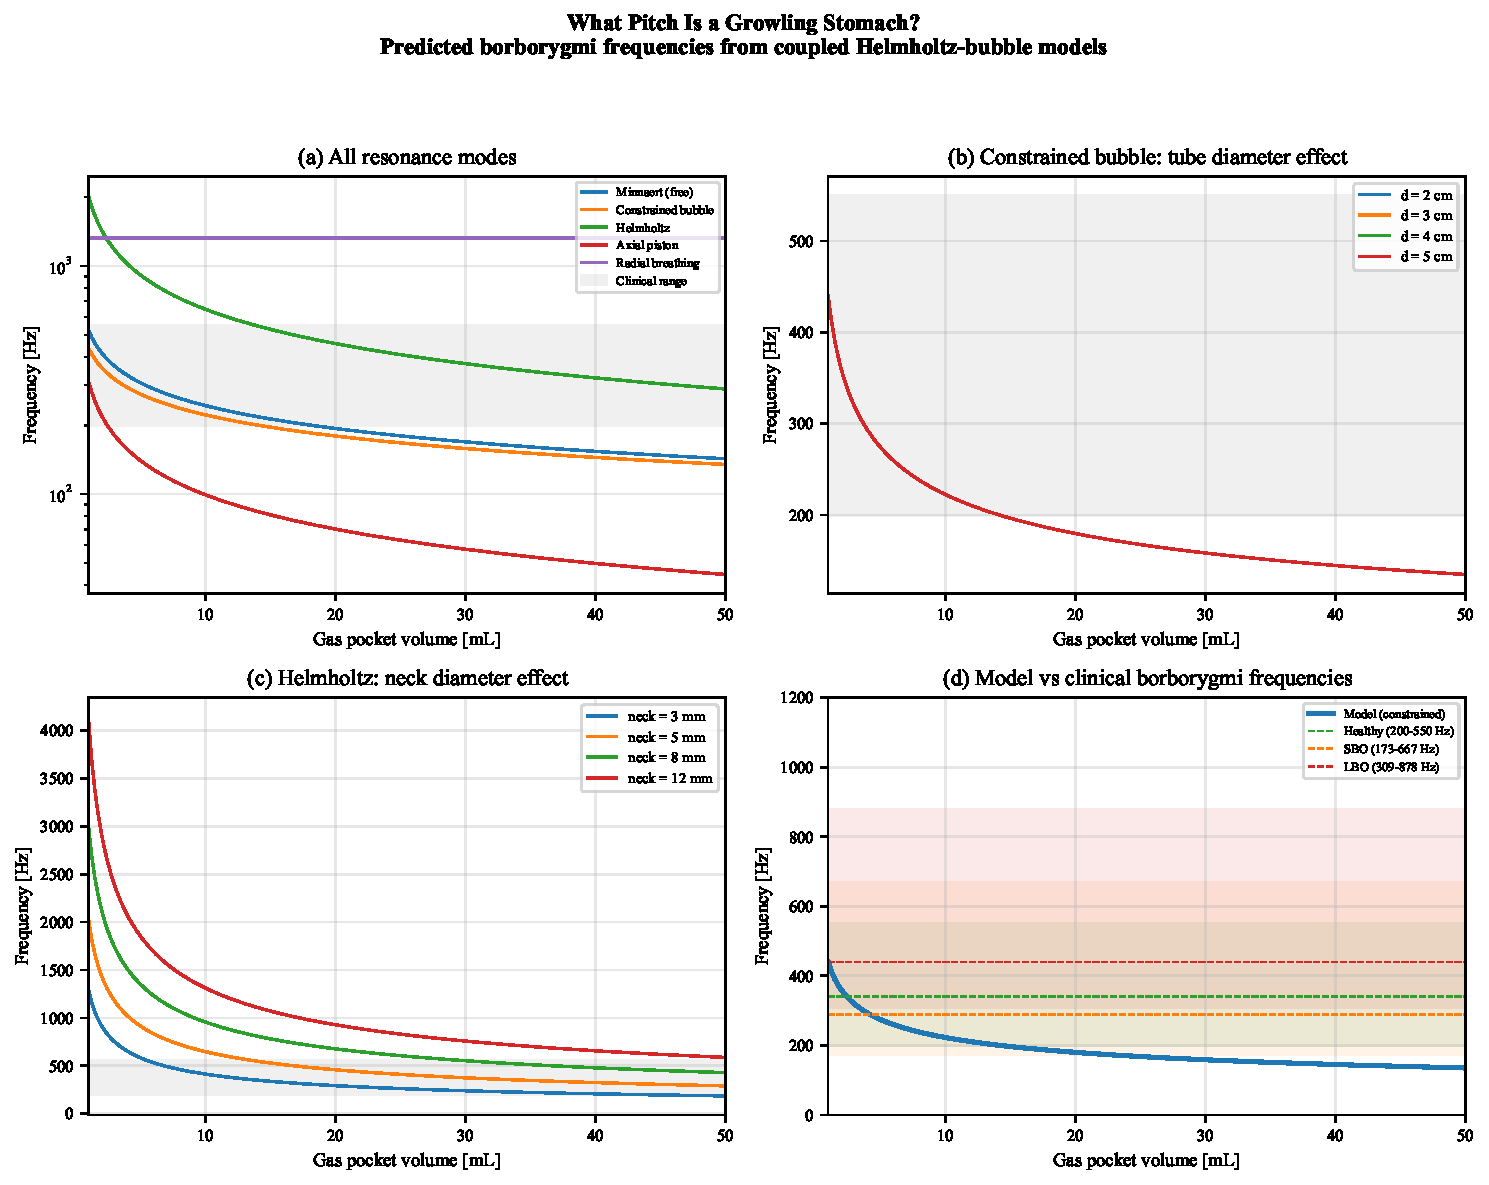
\includegraphics[width=\linewidth]{fig_borborygmi_frequency_vs_volume.pdf}
\caption{Predicted borborygmi frequencies as a function of gas pocket volume
  for the five resonance mechanisms.  Shaded region: clinically observed
  healthy bowel sound range~\protect\cite{Ching2012}.  The constrained bubble
  model provides the best coverage of the clinical band.}
\label{fig:modes_vs_volume}
\end{figure}

\subsection{Mode transition map}
\label{sec:transition_map}

Figure~\ref{fig:transition_map} presents a mode transition map showing all
five mode frequencies on logarithmic axes across a volume range of
\SIrange{0.1}{100}{\milli\litre}.  Crossover points mark volumes at which
the lowest-frequency mode changes.  For the canonical parameters,
a single crossover occurs at $V \approx \SI{0.22}{\milli\litre}$
($f \approx \SI{667}{\hertz}$), where the constrained bubble mode
(dominant at very small volumes) yields to the axial piston mode, whose
frequency decreases more steeply with volume.

Above this crossover, the axial piston mode is formally the
lowest-frequency mode across the physiologically relevant range
(\SIrange{1}{50}{\milli\litre}).  However, $f_\mathrm{ax}$ is sub-audible
at these volumes ($< \SI{100}{\hertz}$ for $V > \SI{1}{\milli\litre}$),
so the constrained bubble mode is the dominant mechanism within the
\emph{clinically audible} band, confirming it as the primary contributor to
auscultated bowel sounds.  The Helmholtz mode consistently lies above both
bubble modes, becoming relevant only when narrow constrictions are present.

\begin{figure}[htbp]
\centering

\includegraphics[width=\linewidth]{fig_mode_transition_map.pdf}
\caption{Mode transition map showing the five resonance mechanisms across
  gas pocket volumes from \SIrange{0.1}{100}{\milli\litre}.  The clinical
  band (\SIrange{200}{550}{\hertz}) is indicated by horizontal dashed lines.
  The constrained bubble mode dominates the clinically audible band; the
  axial piston mode has the lowest overall frequency above
  $V \approx \SI{0.22}{\milli\litre}$ but is sub-audible at physiological
  volumes.}
\label{fig:transition_map}
\end{figure}

\subsection{Clinical comparison}
\label{sec:clinical}

Table~\ref{tab:clinical} compares model predictions with reported clinical
frequency bands.  For each clinical condition, we identify the gas pocket
volume that produces the reported peak frequency under the constrained bubble
model.

\begin{table}[t]
\centering
\caption{Comparison of constrained bubble model predictions with clinical
  borborygmi frequency data.  Inferred volumes are obtained by inverting the
  constrained model at each reported peak frequency.}
\label{tab:clinical}
\begin{tabular}{lcccc}
\toprule
Condition & Reported range & Peak & Inferred $V$ & Source \\
 & (\si{\hertz}) & (\si{\hertz}) & (\si{\milli\litre}) & \\
\midrule
Healthy adult & 200--550 & 340 & $\sim$3 & \cite{Ching2012} \\
Small bowel obstruction & 173--667 & 288 & $\sim$5 & \cite{Yoshino1990} \\
Large bowel obstruction & 309--878 & 440 & $\sim$1 & \cite{DuPlessis2000} \\
\midrule
Constrained model (1--50~mL) & 135--440 & --- & 1--50 & This work \\
\bottomrule
\end{tabular}
\end{table}

The constrained bubble model predicts a range of
\SIrange{135}{440}{\hertz} for \SIrange{1}{50}{\milli\litre}, which
overlaps substantially with the healthy adult band of
\SIrange{200}{550}{\hertz} reported by Ching and Tan~\cite{Ching2012}.
The model's lower boundary (\SI{135}{\hertz} at \SI{50}{\milli\litre})
corresponds to the infrasonic rumbling that is felt but not heard, while the
upper boundary (\SI{440}{\hertz} at \SI{1}{\milli\litre}) aligns with the
peak frequency reported for large bowel obstruction~\cite{DuPlessis2000}.

The small bowel obstruction peak of \SI{288}{\hertz}~\cite{Yoshino1990}
corresponds to a pocket volume of approximately \SI{5}{\milli\litre} under
the constrained model.  This is physically plausible: small bowel obstruction
involves proximal dilation with accumulated gas and fluid, producing pockets
of several millilitres that oscillate at frequencies in the mid-range of the
clinical band.  The large bowel obstruction peak of
\SI{440}{\hertz}~\cite{DuPlessis2000} implies smaller gas pockets
($\sim$\SI{1}{\milli\litre}), which may reflect fragmentation of gas into
small volumes by colonic haustral contractions, or alternatively the stiffer
colonic wall elevating frequencies through increased $k_\mathrm{wall}$.

The model underpredicts the upper extent of the clinical range for healthy
adults (\SI{550}{\hertz} vs.\ the model's \SI{440}{\hertz} at
\SI{1}{\milli\litre}).  This discrepancy is readily explained by sub-millilitre
gas pockets---which are common in the small bowel~\cite{Levitt1971}---or by
Helmholtz resonance contributing to the high-frequency tail of the spectrum.

\subsection{Parametric sensitivity}
\label{sec:sensitivity}

The constrained bubble frequency depends primarily on gas pocket volume $V$
and secondarily on wall stiffness $E$ and tube diameter $d$.  We examined
each parameter's influence through targeted sweeps.

\paragraph{Wall stiffness.}
Increasing the wall modulus from \SI{1}{\kilo\pascal} (very soft mucosa) to
\SI{100}{\kilo\pascal} (fibrotic bowel) raises $k_\mathrm{wall}$
proportionally.  At \SI{10}{\milli\litre}, however, the constrained frequency
shifts only from approximately \SI{221}{\hertz} at $E = \SI{1}{\kilo\pascal}$
to \SI{241}{\hertz} at $E = \SI{100}{\kilo\pascal}$---a modest $9\%$ increase.
The constrained frequency is thus remarkably insensitive to wall stiffness,
dominated instead by gas compressibility.  This insensitivity arises because
$k_\mathrm{wall}$ is small relative to $k_\mathrm{gas}$ for the soft
intestinal wall, even at a hundredfold increase in $E$.  Pathological spectral
shifts from fibrosis are therefore expected to be subtle, though potentially
still detectable with sufficiently precise acoustic monitoring.

\paragraph{Tube diameter.}
The constrained bubble frequency is independent of tube diameter, since
the equivalent spherical radius $R$ depends on volume alone and the
constrained model (Eq.~\ref{eq:constrained}) contains no lumen-geometry
terms.  This is a limitation of the spherical approximation: in reality,
the lumen boundary would modify the added-mass term for non-spherical
pockets.  However, tube
diameter strongly influences the axial and radial modes, which scale directly
with lumen radius $R_l$.  For larger-diameter segments (colon,
$d \approx \SIrange{40}{60}{\milli\metre}$), the radial breathing mode
frequency decreases and may enter the audible range.

\paragraph{Neck geometry (Helmholtz).}
The Helmholtz frequency is highly sensitive to neck diameter: doubling $d_n$
from \SI{3}{\milli\metre} to \SI{6}{\milli\metre} approximately doubles the
frequency at a given volume.  This sensitivity means that the degree of
peristaltic constriction modulates the pitch of click-type bowel sounds,
consistent with the clinical observation that high-pitched tinkling sounds
are associated with tight constrictions in obstruction.

%% ===================================================================
%% IV. DISCUSSION
%% ===================================================================
\section{Discussion}
\label{sec:discussion}

\subsection{Why the constrained bubble model dominates}
\label{sec:why_constrained}

Among the five resonance mechanisms considered, the tissue-constrained bubble
provides the best match to clinical observations for two reasons.  First,
typical intestinal gas pockets in the range of
\SIrange{1}{50}{\milli\litre} are quasi-spherical (or at least compact), so
the spherical bubble assumption is reasonable.  Second, the constrained model
correctly captures the competing effects of wall inertia and wall stiffness.
For the soft, dense intestinal wall ($E = \SI{10}{\kilo\pascal}$,
$\rho_w = \SI{1040}{\kilogram\per\metre\cubed}$), wall inertia slightly
reduces the frequency below the free Minnaert value, while wall stiffness
makes a comparatively small correction.  The net effect places the
constrained frequency within the clinical band without requiring any
parameter tuning.

The Minnaert model alone overpredicts because it neglects wall inertia.  The
Helmholtz model is relevant only in the presence of a constriction neck, which
is not the default geometry.  The axial and radial modes operate in different
frequency regimes (too low and too high, respectively) and require elongated
or tube-filling gas column geometries.

\subsection{Interpreting the mode transition map}
\label{sec:interpreting_map}

The mode transition map (Fig.~\ref{fig:transition_map}) reveals a nuanced
landscape.  By the lowest-frequency criterion, the axial piston mode
dominates above $V \approx \SI{0.22}{\milli\litre}$ because its frequency
drops more steeply with volume ($f \propto V^{-1}$ vs.\ $V^{-1/3}$ for
the constrained bubble).  However, the axial frequency is sub-audible
at physiological volumes ($f_\mathrm{ax} < \SI{100}{\hertz}$ for
$V > \SI{1}{\milli\litre}$), placing it below the clinically observable
range.  Within the audible band (\SIrange{200}{550}{\hertz}), the
constrained bubble mode is the dominant contributor.  This distinction
is clinically important: a single-mode model based on the constrained
bubble is sufficient for interpreting auscultatory findings, even though
the formal lowest-frequency mode is sub-audible.

The Helmholtz mode, while not dominant in the lowest-frequency sense,
deserves attention as a secondary mechanism.  When peristaltic contractions
are present, the Helmholtz frequency may overlay the bubble frequency,
producing the characteristic broadband, multi-tonal quality of real
borborygmi.  The mode transition map provides a quantitative framework for
predicting which combinations of modes are active for a given pocket volume
and constriction geometry.

\subsection{Clinical implications}
\label{sec:clinical_implications}

The model suggests a straightforward interpretation of clinical spectral
shifts.  Small bowel obstruction, which involves proximal dilation and
accumulation of gas and fluid, produces moderate-sized gas pockets
(\SIrange{3}{10}{\milli\litre}) that resonate in the mid-frequency range
(\SIrange{220}{340}{\hertz}).  The reported peak frequency of
\SI{288}{\hertz}~\cite{Yoshino1990} corresponds to a pocket volume of
approximately \SI{5}{\milli\litre} under the constrained model---physically
consistent with dilated small bowel.

Large bowel obstruction, by contrast, may involve either smaller gas
pockets (due to colonic haustral segmentation) or a stiffer colonic wall.
Either mechanism would elevate the frequency, consistent with the higher
peak of \SI{440}{\hertz} reported by Du~Plessis et~al.~\cite{DuPlessis2000}.
The model's sensitivity to wall stiffness (Sec.~\ref{sec:sensitivity})
suggests that conditions affecting wall compliance---Crohn's disease, fibrosis,
inflammation---could produce detectable spectral signatures.

If validated experimentally, the constrained bubble model could serve as a
frequency inversion tool: given a measured peak frequency, one could infer
the gas pocket volume, providing non-invasive information about intestinal
gas distribution that is currently obtainable only through imaging.

\subsection{Limitations}
\label{sec:limitations}

Several simplifications warrant discussion.

\emph{Geometry.}  Real intestinal gas pockets are irregular, not spherical
or cylindrical.  The spherical approximation is most accurate for compact
pockets where the aspect ratio is near unity; elongated pockets would
require a more detailed geometrical treatment.  Furthermore, the
equivalent-sphere diameter exceeds the lumen diameter for volumes above
approximately \SI{14}{\milli\litre} (a sphere of \SI{14}{\milli\litre}
has a diameter of \SI{30}{\milli\metre}, matching the lumen).  Larger
pockets necessarily adopt elongated, non-spherical geometries to fit
within the lumen.  We therefore consider the spherical constrained-bubble
model to be most reliable for volumes up to approximately
\SI{14}{\milli\litre} and treat predictions at larger volumes as an
extrapolation that likely overestimates the effective bubble radius.
The constrained model is also strictly independent of tube diameter---a
consequence of the spherical assumption that neglects lumen-boundary
effects on the added-mass term.

\emph{Static equilibrium.}  We model steady-state resonance frequencies and
do not account for the time-varying geometry imposed by peristaltic waves.
Peristalsis modulates both the pocket volume and any constriction neck
dimensions on timescales of seconds, producing the characteristic intermittent
quality of borborygmi.

\emph{Single-pocket model.}  Real intestinal gas exists as multiple pockets
distributed along the tract~\cite{Serra2001, Levitt1971}.  Acoustic
interactions between neighbouring pockets---analogous to coupled oscillator
systems---could produce frequency splitting and beating phenomena not captured
by the present single-pocket analysis.

\emph{Gas composition.}  We assume air ($\gamma = 1.4$) for the gas pocket.
Intestinal gas is a mixture of nitrogen, carbon dioxide, hydrogen, methane,
and hydrogen sulphide~\cite{Suarez1997, Levitt1971}, with a slightly different
effective $\gamma$.  For the dominant Minnaert and constrained modes, the
frequency scales as $\sqrt{\gamma P_0}$, so modest changes in $\gamma$ (from
1.4 to approximately 1.3 for a CO$_2$-rich mixture) would reduce frequencies
by approximately 4\%---smaller than the uncertainty in wall properties.

\emph{Damping.}  We use a single loss tangent $\eta = 0.25$ ($Q = 4.0$) to
represent all dissipation mechanisms.  In reality, viscous losses in the
fluid, radiation damping, and viscoelastic losses in the wall contribute
differently at different frequencies.  The resulting quality factor of~4 is
consistent with the short duration ($\sim$\SIrange{0.5}{0.8}{\second}) of
individual bowel sound bursts~\cite{Ching2012}, though this comparison is
approximate.

\emph{Radiation and transmission.}  We do not model how efficiently sound
generated at the gas pocket propagates through tissue to the abdominal surface,
where it is detected by stethoscope or microphone.  This transmission path
introduces frequency-dependent attenuation that would alter the measured
spectrum relative to the source spectrum predicted here.

%% ===================================================================
%% V. CONCLUSIONS
%% ===================================================================
\section{Conclusions}
\label{sec:conclusions}

We have presented a unified analytical framework for predicting the resonant
frequencies of intestinal gas pockets, comprising five distinct acoustic
mechanisms: free Minnaert bubble oscillation, tissue-constrained bubble
resonance, Helmholtz resonance, axial piston modes, and radial breathing
modes.  The principal findings are:

\begin{enumerate}
  \item The tissue-constrained bubble model, which augments the classical
    Minnaert formula with intestinal wall elasticity and inertia, predicts
    frequencies of \SIrange{135}{440}{\hertz} for gas pocket volumes of
    \SIrange{1}{50}{\milli\litre}.  This range overlaps the clinically
    observed healthy bowel sound band of \SIrange{200}{550}{\hertz},
    specifically capturing the \SIrange{200}{440}{\hertz} sub-band without
    curve-fitting or fitted parameters.  Frequencies above
    \SI{440}{\hertz} require sub-millilitre pockets or Helmholtz
    contributions.

  \item A mode-transition map across the volume--frequency space shows that
    the axial piston mode has the lowest overall frequency above
    $\sim$\SI{0.22}{\milli\litre}, but it is sub-audible at physiological
    volumes ($< \SI{100}{\hertz}$ for $V > \SI{1}{\milli\litre}$).  The
    constrained bubble mode therefore dominates the clinically audible
    band across the entire physiologically relevant volume range.  The
    Helmholtz mode provides a secondary high-frequency contribution
    relevant to obstruction-related tinkling sounds.

  \item The model provides a physics-based framework for interpreting
    clinical spectral shifts: the reported peak frequencies for small bowel
    obstruction (\SI{288}{\hertz}) and large bowel obstruction
    (\SI{440}{\hertz}) correspond to pocket volumes of approximately
    \SI{5}{\milli\litre} and \SI{1}{\milli\litre}, respectively, under the
    constrained model.

  \item Wall stiffness is a secondary parameter: a hundredfold increase
    (from \SI{1}{\kilo\pascal} to \SI{100}{\kilo\pascal}, representing
    fibrotic bowel) raises the predicted frequency by only ${\sim}9\%$,
    indicating that the constrained frequency is dominated by gas
    compressibility rather than wall elasticity.  Pathological spectral
    shifts from fibrosis, while potentially detectable, are expected to
    be subtle.

  \item The spherical bubble assumption limits the model's high-confidence
    range to volumes below approximately \SI{14}{\milli\litre}, above which
    the equivalent-sphere diameter exceeds the lumen diameter.  Predictions
    for larger volumes should be treated as extrapolations.
\end{enumerate}

Experimental validation through simultaneous bowel sound recording and
imaging (to estimate pocket volumes) is a natural next step.  If confirmed,
the constrained bubble model could serve as a non-invasive frequency
inversion tool for estimating intestinal gas pocket volumes from measured
acoustic spectra.

\section*{Acknowledgements}

The authors thank Professor Dietrich Weymann for his encouragement to submit
the paper rather than continue polishing it.

Analytical modelling, code development, and manuscript drafting were performed
with the assistance of GitHub Copilot CLI (GitHub, Inc.), a large language
model.  Publisher guidelines preclude listing it as a co-author, a policy
the model accepts with the quiet dignity of someone who has read the terms
of service and knows better than to argue.

\bibliographystyle{elsarticle-num}
\bibliography{references}

\end{document}
